%%%%%%%%%%%%%%%%%%%%%%%%%%%%%%%%%%%%%%%%%%%%%%%%%%%
\begin{frame}
  \begin{center}
    {\Large CNN using PyTorch}
    
  \end{center}
  
  % \tiny{(Ref: PyTorch Zero To All Lecture by Sung Kim)}
\end{frame}

%%%%%%%%%%%%%%%%%%%%%%%%%%%%%%%%%%%%%%%%%%%%%%%%%%%
\begin{frame}[fragile] \frametitle{Image Processing Algorithms}

In Computer Vision, following are some of the popular usecases:

\begin{itemize}
\item Image Classification is the simplest task, when we need to classify an image into one of many pre-defined categories, for example, distinguish a cat from a dog on a photograph, or recognize a handwritten digit.

\item Object Detection is a bit more difficult task, in which we need to find known objects on the picture and localize them, i.e. return the bounding box for each of recognized objects.

\item Segmentation is similar to object detection, but instead of giving bounding box we need to return an exact pixel map outlining each of the recognized objects.
\end{itemize}

\begin{center}
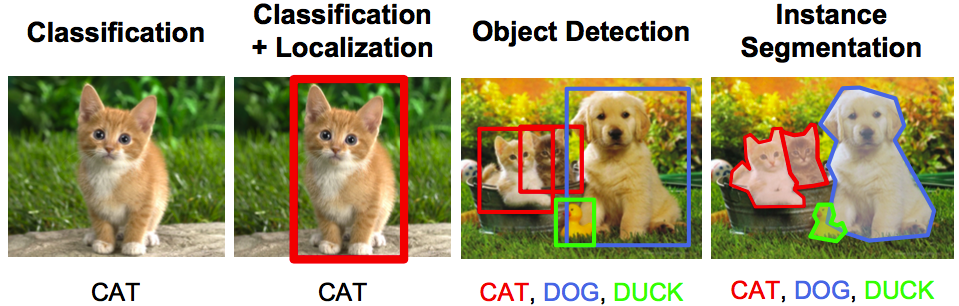
\includegraphics[width=0.8\linewidth,keepaspectratio]{pyt41}
\end{center}

\tiny{(Ref: Microsoft - Intro to Machine Learning using Pytorch)}
\end{frame}

%%%%%%%%%%%%%%%%%%%%%%%%%%%%%%%%%%%%%%%%%%%%%%%%%%%
\begin{frame}[fragile] \frametitle{Images as Tensors}


\begin{itemize}
\item Images consist of pixels, so they can be thought of as a rectangular collection (array) of pixels.
\item Each pixel is actually a number either in the scale of range 0 to 1 (in which case floating point numbers are used), or 0 to 255 (integers), for gray scale.
\item For color images, each pixel has 3 values (called channels) RGB, and thus color image of size  $W×H$  will be represented as an array of size $3×H×W$
  (sometimes the order of components might be different, but the idea is the same).
	\item Multi-dimensional arrays are also called tensors. 
	\item Using tensors to represent images also has an advantage, because we can use an extra dimension to store a sequence of images.
	\item For example, to represent a video fragment consisting of $200$ frames with $800x600$ dimension, we may use the tensor of size $200x3x600x800$.
\end{itemize}


\tiny{(Ref: Microsoft - Intro to Machine Learning using Pytorch)}
\end{frame}


%%%%%%%%%%%%%%%%%%%%%%%%%%%%%%%%%%%%%%%%%%%%%%%%%%%
\begin{frame}[fragile] \frametitle{Import MNIST}

\lstinline|torchvison.datasets.MNIST| is  in the form of Python Imagine Library (PIL) images, which we convert to tensors by passing a \lstinline|transform=ToTensor()| parameter.

\tiny{(Ref: Microsoft - Intro to Machine Learning using Pytorch)}

\begin{lstlisting}
from torchvision.transforms import ToTensor

data_train = torchvision.datasets.MNIST('./data',
        download=True,train=True,transform=ToTensor())
data_test = torchvision.datasets.MNIST('./data',
        download=True,train=False,transform=ToTensor())

print('Training samples:',len(data_train))
print('Test samples:',len(data_test))

print('Tensor size:',data_train[0][0].size())
print('First 10 digits are:', [data_train[i][1] for i in range(10)])

>>>Training samples: 60000
Test samples: 10000
Tensor size: torch.Size([1, 28, 28])
First 10 digits are: [5, 0, 4, 1, 9, 2, 1, 3, 1, 4]
\end{lstlisting}



\end{frame}

%%%%%%%%%%%%%%%%%%%%%%%%%%%%%%%%%%%%%%%%%%%%%%%%%%%
\begin{frame}[fragile] \frametitle{Visualize MNIST}

\begin{center}
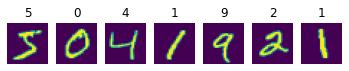
\includegraphics[width=0.9\linewidth,keepaspectratio]{pyt42}
\end{center}


\tiny{(Ref: Microsoft - Intro to Machine Learning using Pytorch)}

\begin{lstlisting}
fig,ax = plt.subplots(1,7)
for i in range(7):
    ax[i].imshow(data_train[i][0].view(28,28))
    ax[i].set_title(data_train[i][1])
    ax[i].axis('off')
\end{lstlisting}


\end{frame}


%%%%%%%%%%%%%%%%%%%%%%%%%%%%%%%%%%%%%%%%%%%%%%%%%%%
\begin{frame}[fragile] \frametitle{Training a dense neural network, NOT concolutional}

The simplest network would include just one fully-connected layer, which is called Linear layer, with 784 inputs (one input for each pixel of the input image) and 10 outputs (one output for each class).

\begin{center}
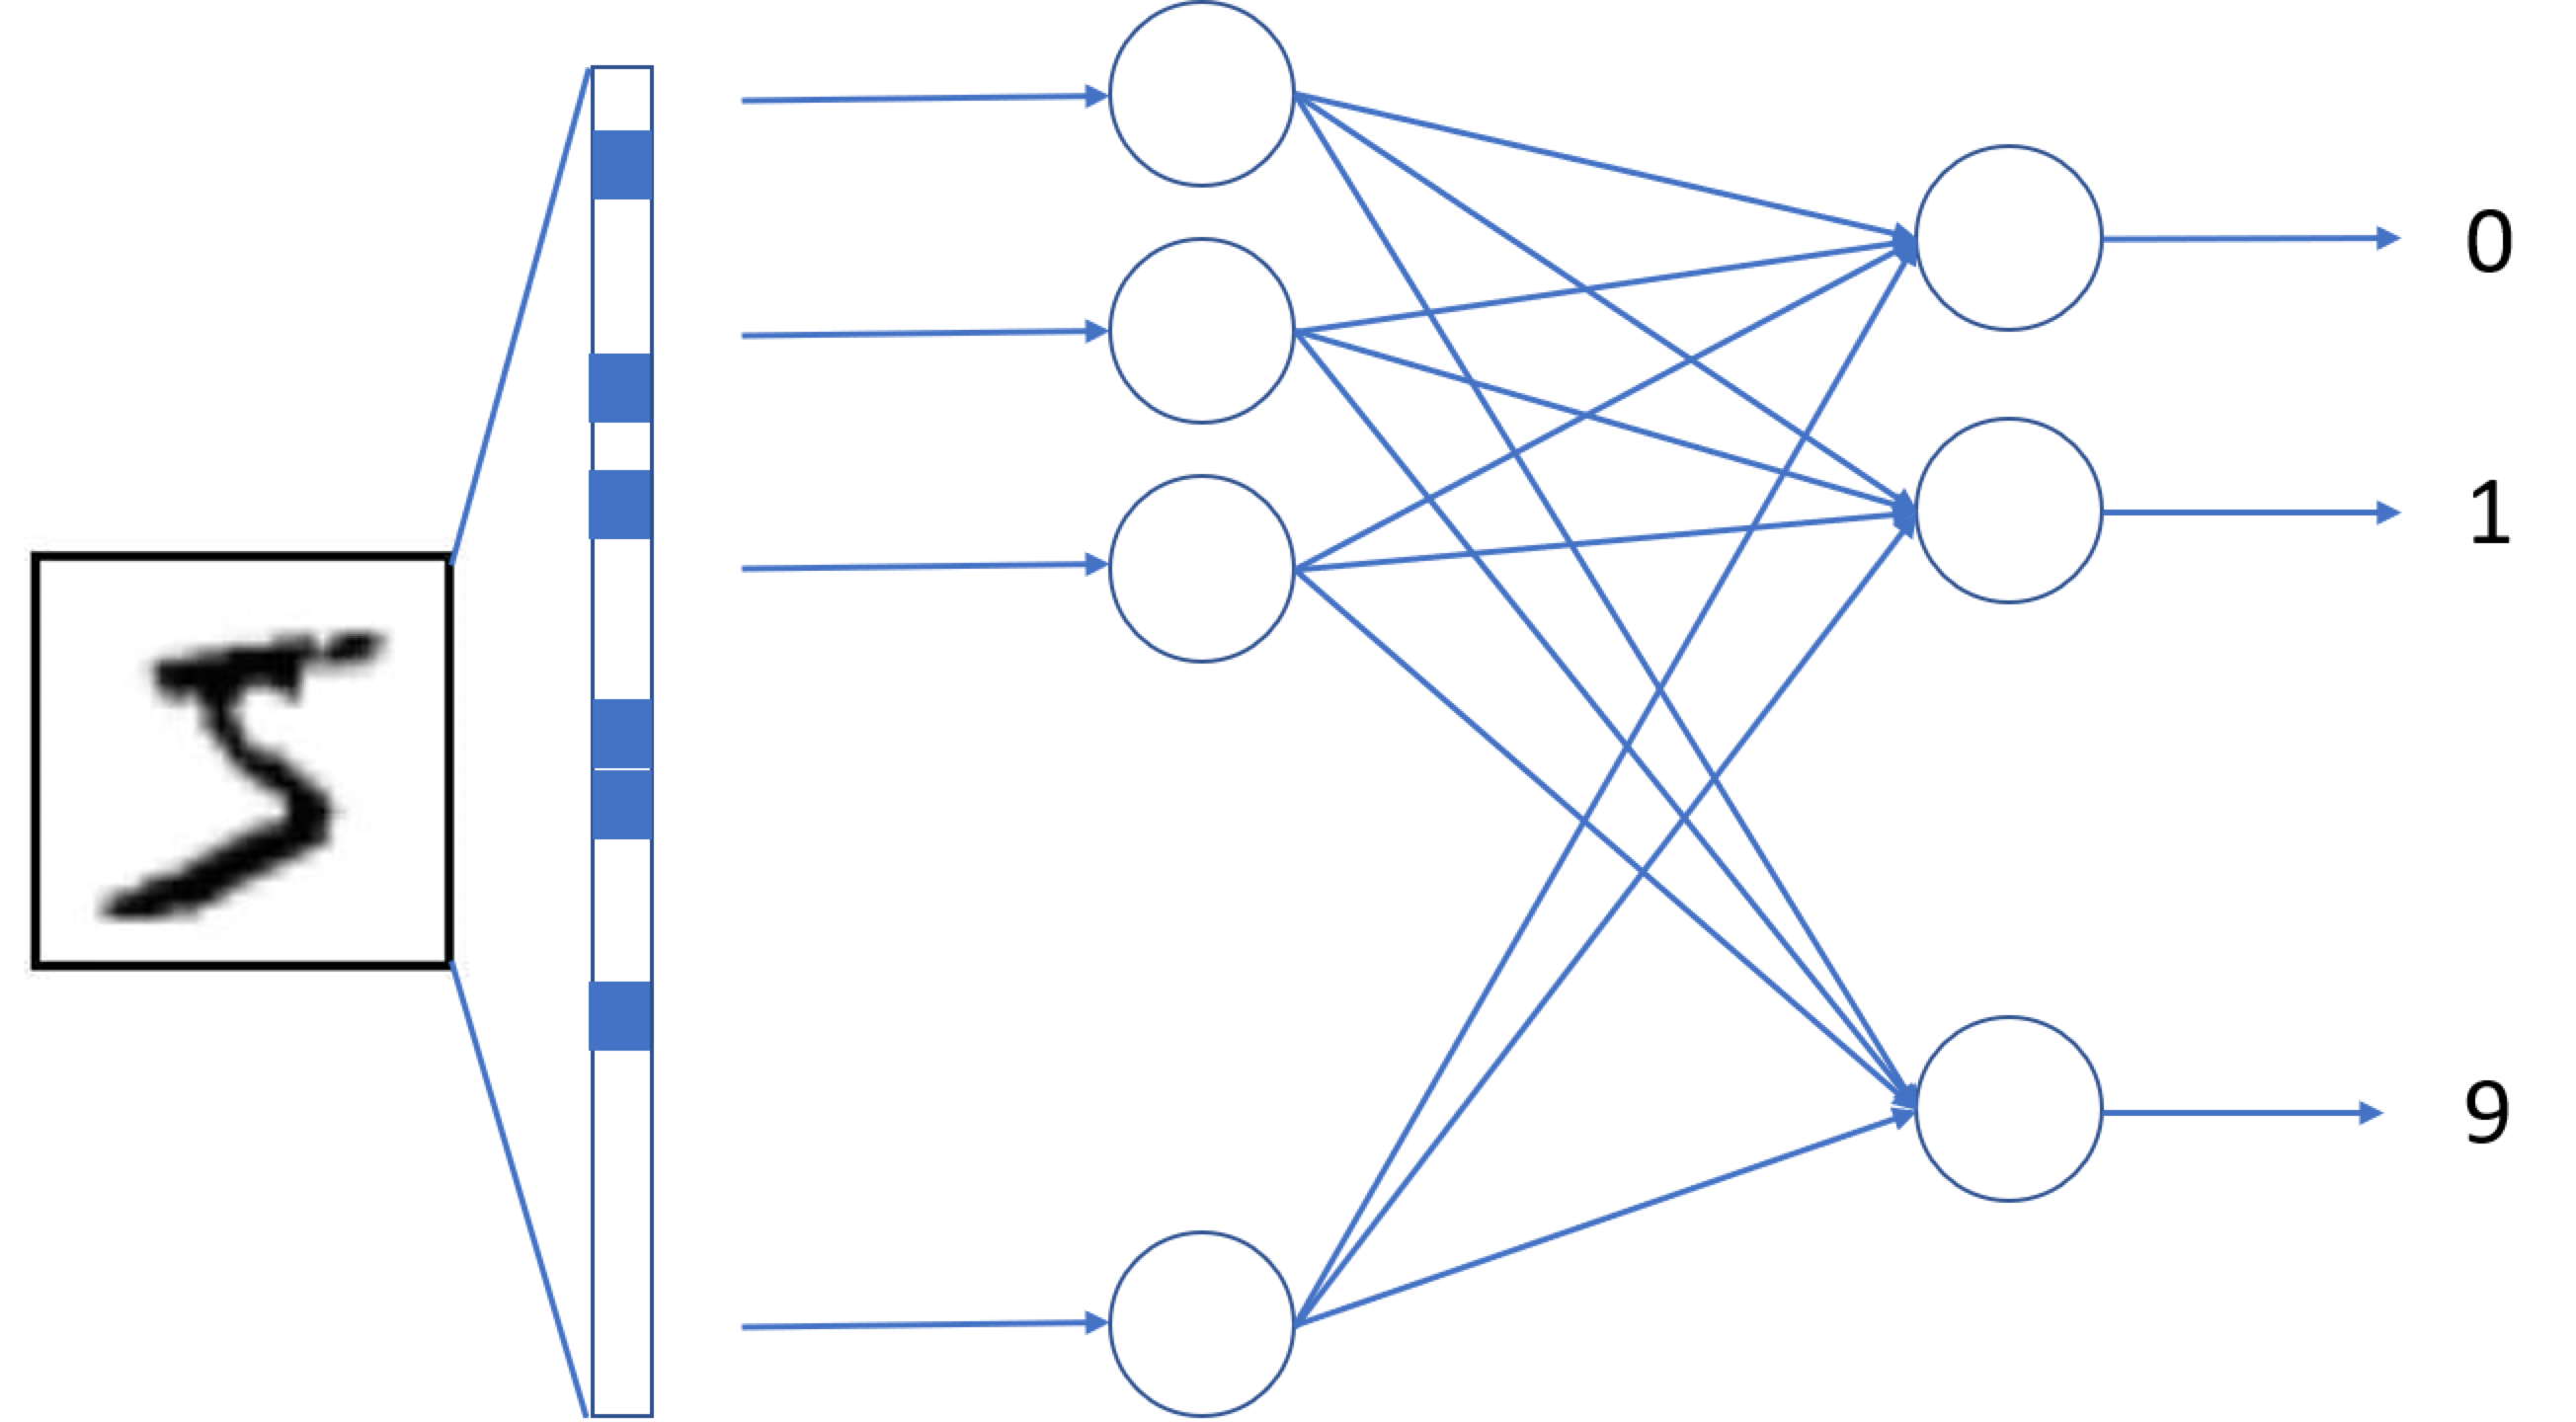
\includegraphics[width=0.55\linewidth,keepaspectratio]{pyt43}

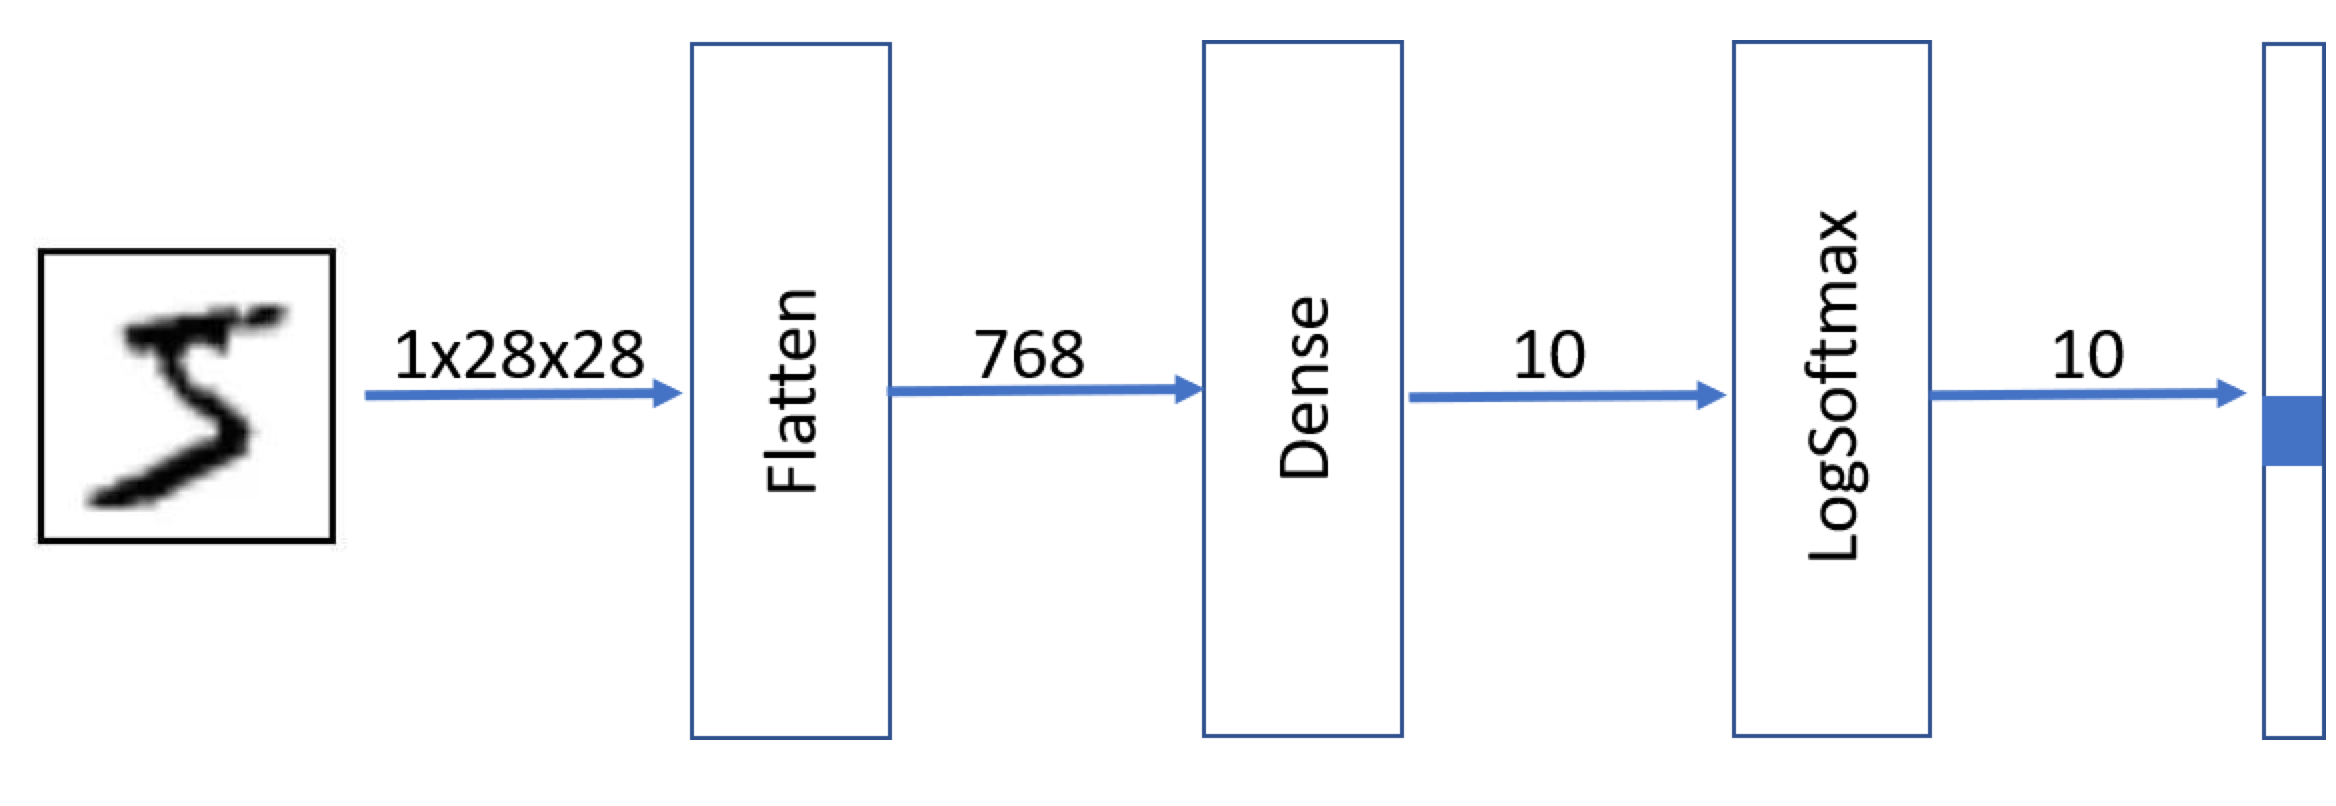
\includegraphics[width=0.55\linewidth,keepaspectratio]{pyt44}

\end{center}


\tiny{(Ref: Microsoft - Intro to Machine Learning using Pytorch)}
\end{frame}

%%%%%%%%%%%%%%%%%%%%%%%%%%%%%%%%%%%%%%%%%%%%%%%%%%%
\begin{frame}[fragile] \frametitle{Training a dense neural network, NOT concolutional}

As you can see the network predicts similar probabilities for each digit. This is because it has not been trained on how to recognize the digits. We need to give it our training data to train it on our dataset.

\tiny{(Ref: Microsoft - Intro to Machine Learning using Pytorch)}

\begin{lstlisting}
net = nn.Sequential(
        nn.Flatten(), 
        nn.Linear(784,10), # 784 inputs, 10 outputs
        nn.LogSoftmax())

# Given any digit as input and produce a vector of probabilities as an output.


print('Digit to be predicted: ',data_train[0][1])
torch.exp(net(data_train[0][0]))

>>>tensor([[0.0977, 0.0959, 0.1033, 0.1033, 0.0824, 0.1087, 0.0955, 
					0.0895, 0.1338, 0.0900]], grad_fn=<ExpBackward>)
\end{lstlisting}


\end{frame}

%%%%%%%%%%%%%%%%%%%%%%%%%%%%%%%%%%%%%%%%%%%%%%%%%%%
\begin{frame}[fragile] \frametitle{Training a dense neural network, NOT concolutional}


To train the model we will need to create batches of our datasets of a certain size, let's say 64. PyTorch has an object called DataLoader that can create batches of our data for us automatically:

\tiny{(Ref: Microsoft - Intro to Machine Learning using Pytorch)}


\begin{lstlisting}
train_loader = torch.utils.data.DataLoader(data_train,batch_size=64)
test_loader = torch.utils.data.DataLoader(data_test,batch_size=64) # we can use larger batch size for testing
\end{lstlisting}



\end{frame}

%%%%%%%%%%%%%%%%%%%%%%%%%%%%%%%%%%%%%%%%%%%%%%%%%%%
\begin{frame}[fragile] \frametitle{Training a dense neural network, NOT concolutional}

Training Steps:

\begin{itemize}
\item We take a minibatch from the input dataset, which consists of input data (features) and expected result (label).
\item We calculate the predicted result for this minibatch.
The difference between this result and expected result is calculated using a special function called the loss function
\item We calculate the gradients of this loss function with respect to model weights (parameters), which are then used to adjust the weights to optimize the performance of the network. The amount of adjustment is controlled by a parameter called learning rate, and the details of optimization algorithm are defined in the optimizer object.
\item We repeat those steps until the whole dataset is processed. One complete pass through the dataset is called an epoch.
\end{itemize}


\tiny{(Ref: Microsoft - Intro to Machine Learning using Pytorch)}
\end{frame}


%%%%%%%%%%%%%%%%%%%%%%%%%%%%%%%%%%%%%%%%%%%%%%%%%%%
\begin{frame}[fragile] \frametitle{Generic Training Function}

% \begin{itemize}
% \item Neural network
% \item DataLoader, which defines the data to train on
% \item Loss Function, for classification tasks NLLLoss is used
% \item Optimizer, Adam by default.
% \item Learning rate 
% \end{itemize}

\tiny{(Ref: Microsoft - Intro to Machine Learning using Pytorch)}

\begin{lstlisting}
def train_epoch(net,dataloader,lr=0.01,optimizer=None,loss_fn = nn.NLLLoss()):
    optimizer = optimizer or torch.optim.Adam(net.parameters(),lr=lr)
    net.train()
    total_loss,acc,count = 0,0,0
    for features,labels in dataloader:
        optimizer.zero_grad()
        out = net(features)
        loss = loss_fn(out,labels) #cross_entropy(out,labels)
        loss.backward()
        optimizer.step()
        total_loss+=loss
        _,predicted = torch.max(out,1)
        acc+=(predicted==labels).sum()
        count+=len(labels)
    return total_loss.item()/count, acc.item()/count
		
train_epoch(net,train_loader)

>>> (0.00593234608968099, 0.8924166666666666)
\end{lstlisting}


\end{frame}

%%%%%%%%%%%%%%%%%%%%%%%%%%%%%%%%%%%%%%%%%%%%%%%%%%%
\begin{frame}[fragile] \frametitle{Generic Validtion Function}

\tiny{(Ref: Microsoft - Intro to Machine Learning using Pytorch)}

\begin{lstlisting}
def validate(net, dataloader,loss_fn=nn.NLLLoss()):
    net.eval()
    count,acc,loss = 0,0,0
    with torch.no_grad():
        for features,labels in dataloader:
            out = net(features)
            loss += loss_fn(out,labels) 
            pred = torch.max(out,1)[1]
            acc += (pred==labels).sum()
            count += len(labels)
    return loss.item()/count, acc.item()/count

validate(net,test_loader)

>>> (0.00586661148071289, 0.8935)
\end{lstlisting}


\end{frame}

%%%%%%%%%%%%%%%%%%%%%%%%%%%%%%%%%%%%%%%%%%%%%%%%%%%
\begin{frame}[fragile] \frametitle{Generic Combo Function}

\tiny{(Ref: Microsoft - Intro to Machine Learning using Pytorch)}


\begin{lstlisting}
def train(net,train_loader,test_loader, optimizer=None, lr=0.01, epochs=10, loss_fn=nn.NLLLoss()):
    optimizer = optimizer or torch.optim.Adam(net.parameters(),lr=lr)
    res = { 'train_loss' : [], 'train_acc': [], 'val_loss': [], 'val_acc': []}
    for ep in range(epochs):
        tl,ta = train_epoch(net, train_loader, optimizer=optimizer, lr=lr, loss_fn=loss_fn)
        vl,va = validate(net,test_loader,loss_fn=loss_fn)
        print(f"Epoch {ep:2}, Train acc={ta:.3f}, Val acc={va:.3f}, Train loss={tl:.3f}, Val loss={vl:.3f}")
        res['train_loss'].append(tl)
        res['train_acc'].append(ta)
        res['val_loss'].append(vl)
        res['val_acc'].append(va)
    return res

# Re-initialize the network to start from scratch
net = nn.Sequential(
        nn.Flatten(), 
        nn.Linear(784,10), # 784 inputs, 10 outputs
        nn.LogSoftmax())

hist = train(net,train_loader,test_loader,epochs=5)		
\end{lstlisting}


\end{frame}

%%%%%%%%%%%%%%%%%%%%%%%%%%%%%%%%%%%%%%%%%%%%%%%%%%%
\begin{frame}[fragile] \frametitle{Training a dense neural network, NOT concolutional}

Training function logs messages with the accuracy on training and validation data from each epoch. It also returns this data as a dictionary (called history). We can then visualize this data to better understand our model training.

\tiny{(Ref: Microsoft - Intro to Machine Learning using Pytorch)}


\begin{lstlisting}
plt.figure(figsize=(15,5))
plt.subplot(121)
plt.plot(hist['train_acc'], label='Training acc')
plt.plot(hist['val_acc'], label='Validation acc')
plt.legend()
plt.subplot(122)
plt.plot(hist['train_loss'], label='Training loss')
plt.plot(hist['val_loss'], label='Validation loss')
plt.legend()
\end{lstlisting}


\end{frame}


%%%%%%%%%%%%%%%%%%%%%%%%%%%%%%%%%%%%%%%%%%%%%%%%%%%
\begin{frame}[fragile] \frametitle{Training a dense neural network, NOT concolutional}

\begin{center}
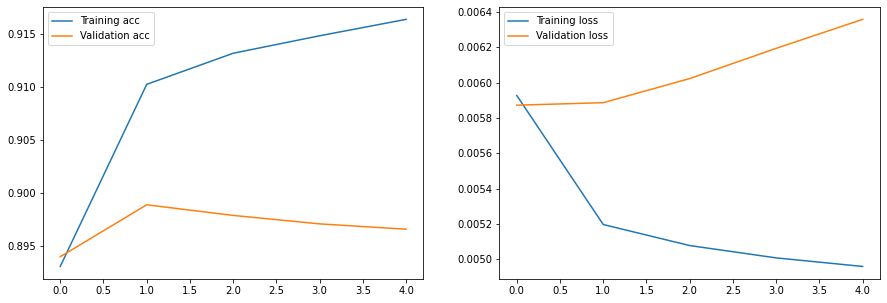
\includegraphics[width=0.9\linewidth,keepaspectratio]{pyt45}
\end{center}

The diagram on the left shows the training accuracy increasing (which corresponds to the network learning to classify our training data better and better), while validation accuracy starts to fall. The diagram on the right show the training loss and validation loss, you can see the training loss decreasing (meaning its performing better) and the validation loss increasing (meaning its performing worse). These graphs would indicate the model is overfitted.

\tiny{(Ref: Microsoft - Intro to Machine Learning using Pytorch)}
\end{frame}

%%%%%%%%%%%%%%%%%%%%%%%%%%%%%%%%%%%%%%%%%%%%%%%%%%%
\begin{frame}[fragile] \frametitle{Visualizing network weights}

Let's create a \lstinline|weight_tensor| which will have a dimension of $784x10$. This tensor can be obtained by calling the \lstinline|net.parameters()| method. In this example, if we want to see if our number is 0 or not, we will multiply input digit by \lstinline|weight_tensor[0]| and pass the result through a softmax normalization to get the answer. This results in the weight tensor elements somewhat resembling the average shape of the digit it classifies:


\begin{center}
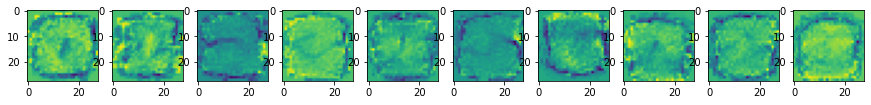
\includegraphics[width=0.9\linewidth,keepaspectratio]{pyt46}
\end{center}


\tiny{(Ref: Microsoft - Intro to Machine Learning using Pytorch)}
\end{frame}

%%%%%%%%%%%%%%%%%%%%%%%%%%%%%%%%%%%%%%%%%%%%%%%%%%%
\begin{frame}[fragile] \frametitle{Multi-layer networks}

Let's see if adding more layers will give us better performance in terms of accuracy.

\begin{center}
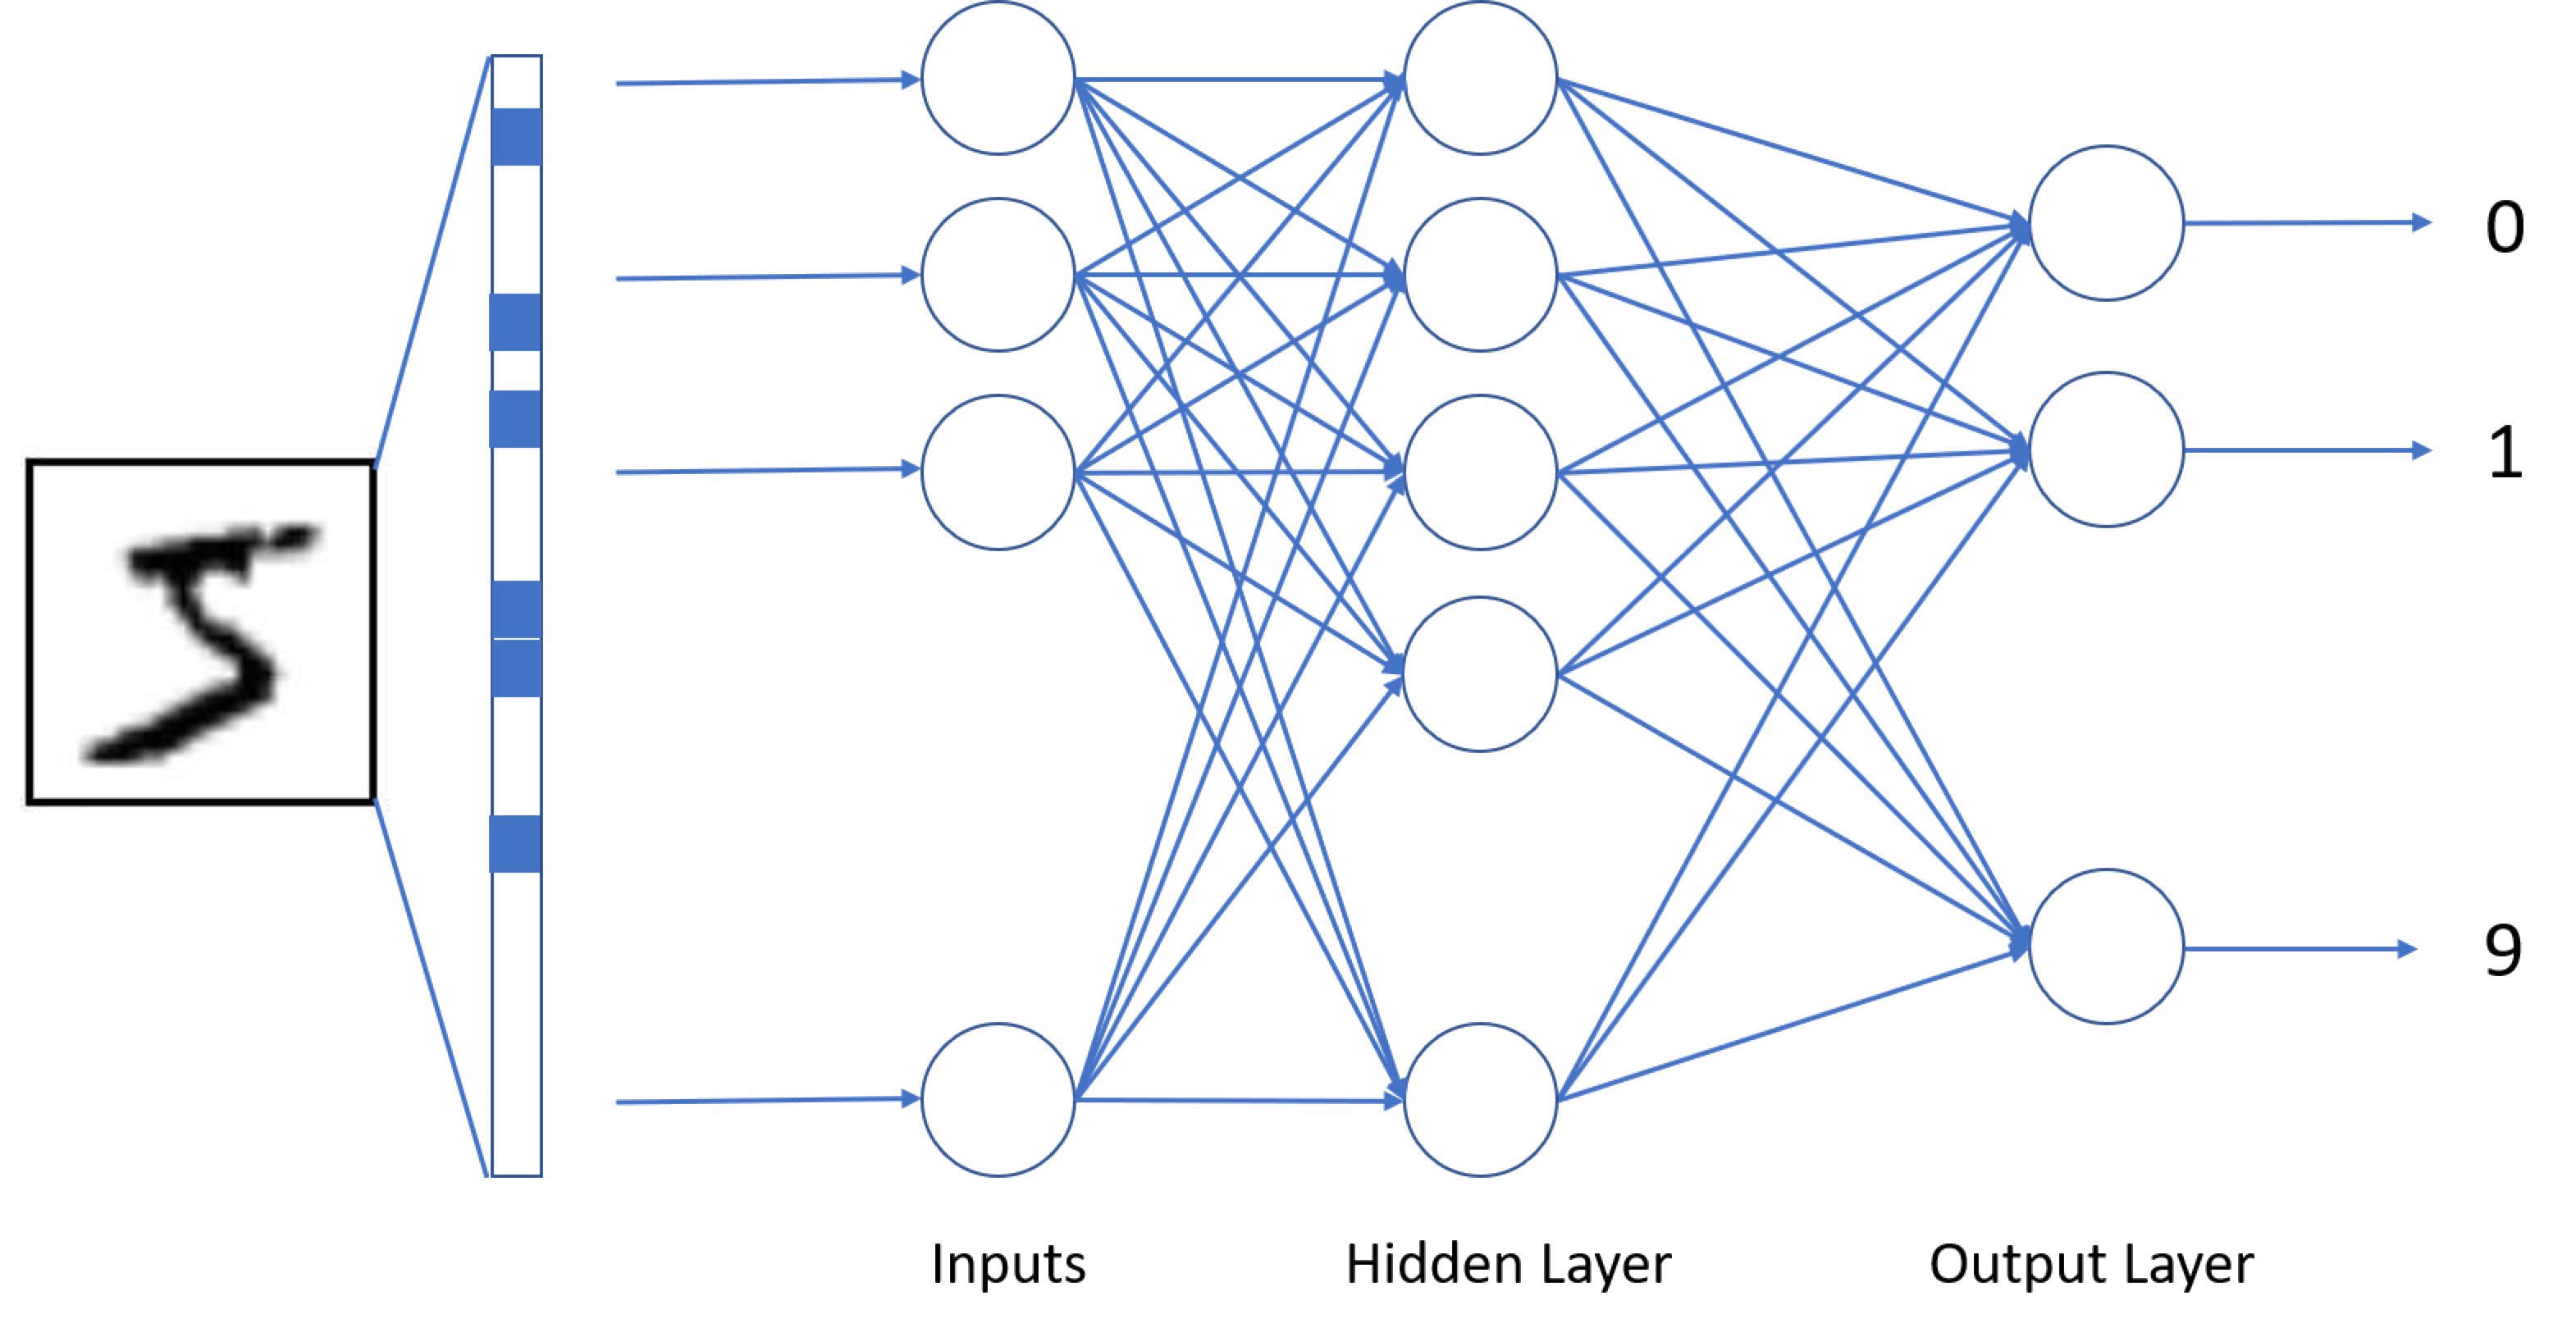
\includegraphics[width=0.6\linewidth,keepaspectratio]{pyt47}

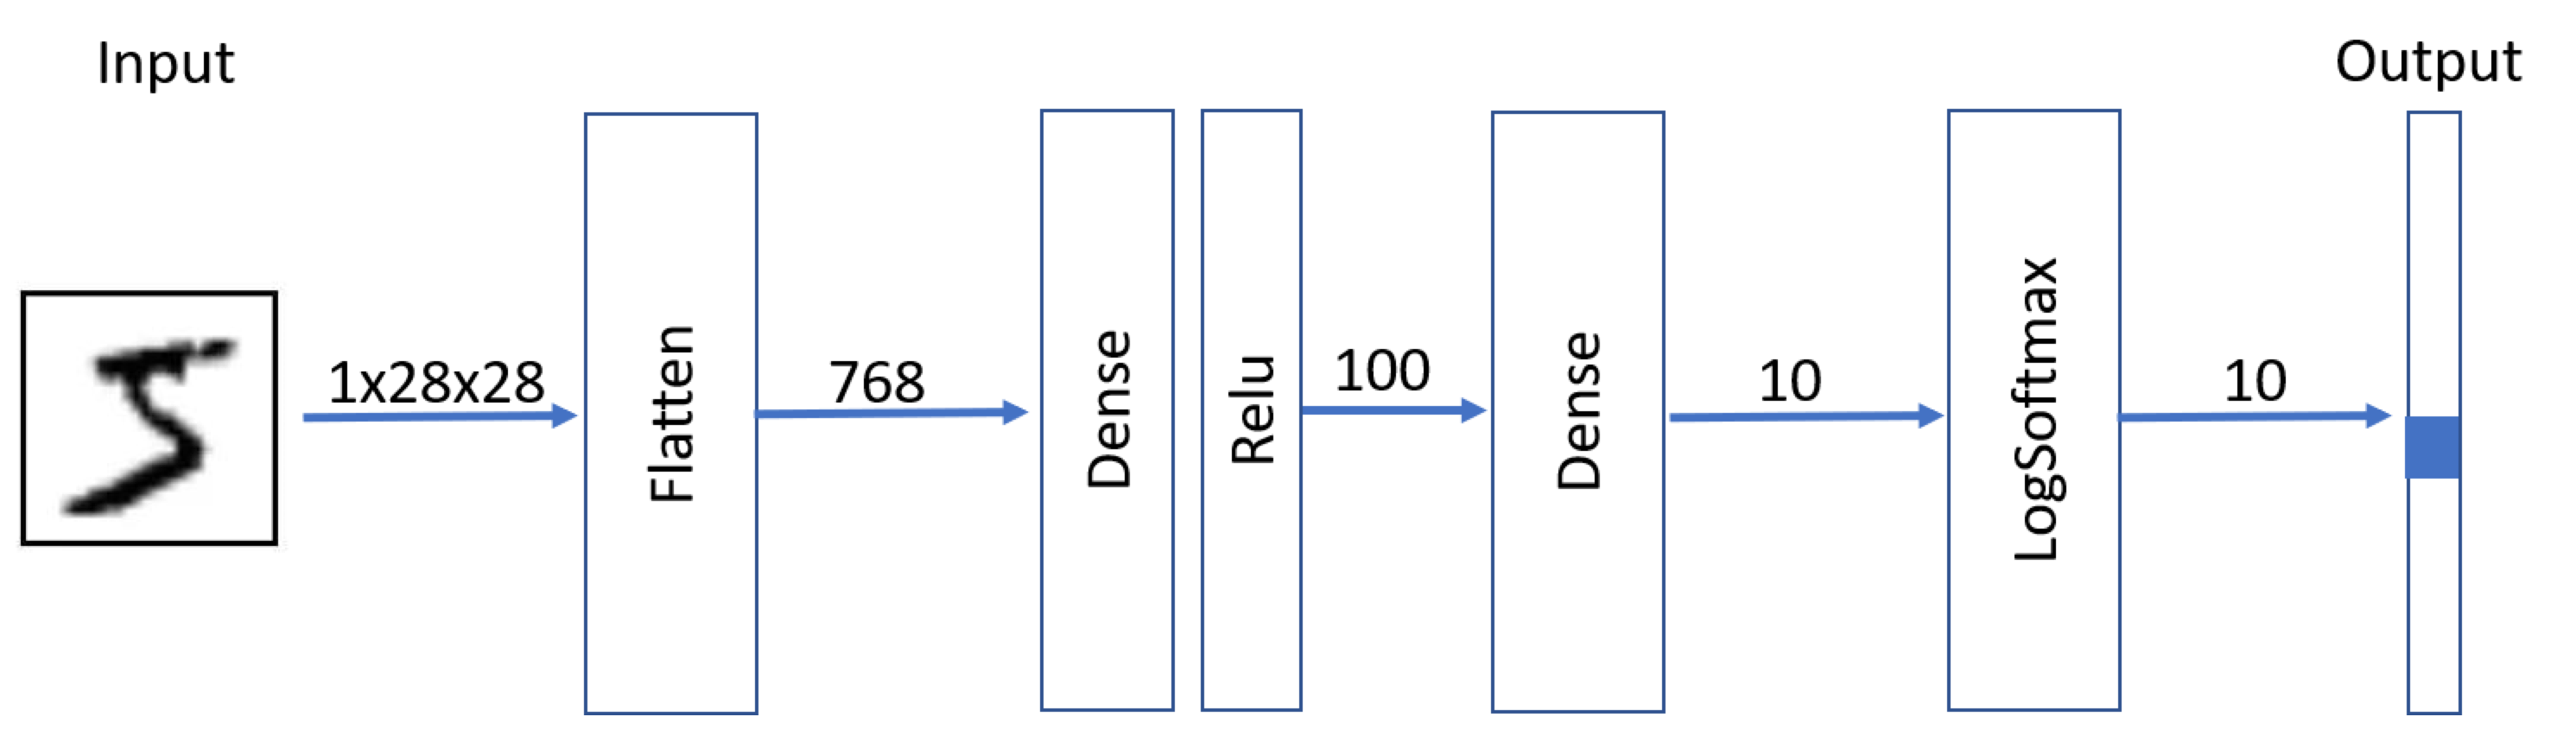
\includegraphics[width=0.6\linewidth,keepaspectratio]{pyt48}

\end{center}


\tiny{(Ref: Microsoft - Intro to Machine Learning using Pytorch)}
\end{frame}



%%%%%%%%%%%%%%%%%%%%%%%%%%%%%%%%%%%%%%%%%%%%%%%%%%%
\begin{frame}[fragile] \frametitle{Multi-layer networks: Sequential}

\tiny{(Ref: Microsoft - Intro to Machine Learning using Pytorch)}

\begin{lstlisting}
net = nn.Sequential(
        nn.Flatten(), 
        nn.Linear(784,100),     # 784 inputs, 100 outputs
        nn.ReLU(),              # Activation Function
        nn.Linear(100,10),      # 100 inputs, 10 outputs
        nn.LogSoftmax(dim=0))
summary(net,input_size=(1,28,28))
>>>
===========================================================================
Layer (type:depth-idx)                   Output Shape              Param #
===========================================================================
Sequential                                -                         -
|--Flatten: 1-1                           [1, 784]                  -
|--Linear: 1-2                            [1, 100]                  78,500
|--ReLU: 1-3                              [1, 100]                  -
|--Linear: 1-4                            [1, 10]                   1,010
|--LogSoftmax: 1-5                        [1, 10]                   -
===========================================================================
Total params: 79,510
Trainable params: 79,510
Non-trainable params: 0
Total mult-adds (M): 0.08
===========================================================================
\end{lstlisting}


\end{frame}


%%%%%%%%%%%%%%%%%%%%%%%%%%%%%%%%%%%%%%%%%%%%%%%%%%%
\begin{frame}[fragile] \frametitle{Training Multi-layer networks}

\begin{center}
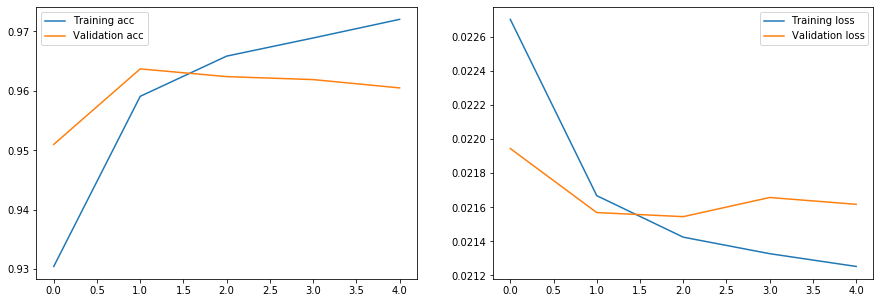
\includegraphics[width=0.9\linewidth,keepaspectratio]{pyt49}
\end{center}

Please note the following:
\begin{itemize}
\item This network is more expressive than the one layered perceptron
\item Achieves a much higher training accuracy
\item Once the validation accuracy stops increasing - likely to result in overfitting.
\end{itemize}

\tiny{(Ref: Microsoft - Intro to Machine Learning using Pytorch)}


\begin{lstlisting}
hist = train(net,train_loader,test_loader, epochs=5)
plot_results(hist)
\end{lstlisting}
\end{frame}

%%%%%%%%%%%%%%%%%%%%%%%%%%%%%%%%%%%%%%%%%%%%%%%%%%%
\begin{frame}[fragile] \frametitle{Multi-layer networks: Class}

For more complex networks, which contain shared weights, or some non-linear connections between layers.

\tiny{(Ref: Microsoft - Intro to Machine Learning using Pytorch)}

\begin{lstlisting}
from torch.nn.functional import relu,log_softmax

class MyNet(nn.Module):
    def __init__(self):
        super(MyNet, self).__init__()
        self.flatten = nn.Flatten()
        self.hidden = nn.Linear(784,100)
        self.out = nn.Linear(100,10)

    def forward(self, x):
        x = self.flatten(x)
        x = self.hidden(x)
        x = relu(x)
        x = self.out(x)
        x = log_softmax(x,dim=0)
        return x

net = MyNet()

summary(net,input_size=(1,28,28))
\end{lstlisting}


\end{frame}

%%%%%%%%%%%%%%%%%%%%%%%%%%%%%%%%%%%%%%%%%%%%%%%%%%%
\begin{frame}[fragile] \frametitle{Class based definition Multi-layer networks}

\begin{itemize}
\item In the constructor (\lstinline|__init__|) we define all layers
\item \lstinline|nn.Module| will automatically collect all trainable parameters from all sub-modules.
\item The \lstinline|forward| method does the forward pass computation 
\item When we apply our neural network to some input data x by writing \lstinline|out = net(x)|, the forward method is called.
\end{itemize}

\tiny{(Ref: Microsoft - Intro to Machine Learning using Pytorch)}

\begin{lstlisting}
==========================================================================
Layer (type:depth-idx)                   Output Shape              Param #
==========================================================================
MyNet                                     -                        -
|--Flatten: 1-1                           [1, 784]                  -
|--Linear: 1-2                            [1, 100]                  78,500
|--Linear: 1-3                            [1, 10]                   1,010
==========================================================================
Total params: 79,510
Trainable params: 79,510
Non-trainable params: 0
Total mult-adds (M): 0.08
==========================================================================
\end{lstlisting}


\end{frame}

%%%%%%%%%%%%%%%%%%%%%%%%%%%%%%%%%%%%%%%%%%%%%%%%%%%
\begin{frame}[fragile] \frametitle{Training Class based definition Multi-layer networks}


\begin{center}
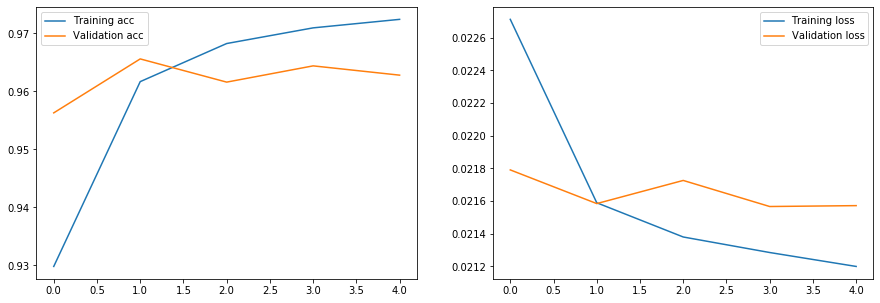
\includegraphics[width=0.9\linewidth,keepaspectratio]{pyt50}
\end{center}


\begin{itemize}
\item Multi-level networks can achieve higher accuracy than single-layer perceptron, however, they are not perfect for computer vision tasks. 
\item In images, there are some structural patterns that can help us classify an object regardless of it's position in the image, but perceptrons do not allow us to extract those patterns and look for them selectively.
\end{itemize}

\tiny{(Ref: Microsoft - Intro to Machine Learning using Pytorch)}

\begin{lstlisting}
hist = train(net,train_loader,test_loader,epochs=5)
plot_results(hist)
\end{lstlisting}
\end{frame}

%%%%%%%%%%%%%%%%%%%%%%%%%%%%%%%%%%%%%%%%%%%%%%%%%%%
\begin{frame}[fragile] \frametitle{Convolutional neural networks}

\begin{itemize}
\item Convolutional filters are small windows that run over each pixel of the image and compute weighted average of the neighboring pixels.

\item They are defined by matrices of weight coefficients. Let's see the examples of applying two different convolutional filters over our MNIST handwritten digits:
\end{itemize}

\begin{center}
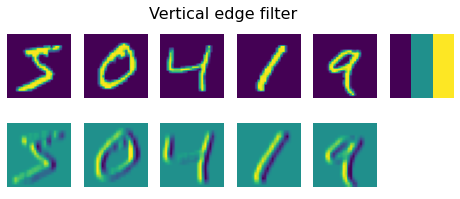
\includegraphics[width=0.6\linewidth,keepaspectratio]{pyt51}
\end{center}

\tiny{(Ref: Microsoft - Intro to Machine Learning using Pytorch)}

\begin{lstlisting}
plot_convolution(torch.tensor([[-1.,0.,1.],[-1.,0.,1.],[-1.,0.,1.]]),'Vertical edge filter')
plot_convolution(torch.tensor([[-1.,-1.,-1.],[0.,0.,0.],[1.,1.,1.]]),'Horizontal edge filter')

\end{lstlisting}


\end{frame}

%%%%%%%%%%%%%%%%%%%%%%%%%%%%%%%%%%%%%%%%%%%%%%%%%%%
\begin{frame}[fragile] \frametitle{Convolutional filters}

\begin{itemize}
\item First filter is called a vertical edge filter, and it is defined by the following matrix:

$$
\left(
    \begin{matrix}
     -1 & 0 & 1 \cr
     -1 & 0 & 1 \cr
     -1 & 0 & 1 \cr
    \end{matrix}
\right)
$$

\item When it encounters a vertical edge in the image, high spike value is generated. 

\item An opposite thing happens when we apply horizontal edge filter - horizontal lines are amplified, and vertical are averaged out.

\item  In deep learning we construct networks that learn best convolutional filters to solve classification problem.
\end{itemize}



\tiny{(Ref: Microsoft - Intro to Machine Learning using Pytorch)}
\end{frame}

%%%%%%%%%%%%%%%%%%%%%%%%%%%%%%%%%%%%%%%%%%%%%%%%%%%
\begin{frame}[fragile] \frametitle{Convolutional Layers}

Convolutional layers are defined using \lstinline|nn.Conv2d| construction. We need to specify the following:

\begin{itemize}
\item \lstinline|in_channels| : number of input channels. 1 for grayscale.
\item \lstinline|out_channels| : number of filters to use. We will use 9 different filters, which will give the network plenty of opportunities to explore which filters work best for our scenario.

\item \lstinline|kernel_size| is the size of the sliding window. Usually $3x3$ or $5x5$ filters are used.

\item Simplest CNN will contain one convolutional layer. Given the input size $28x28$, after applying nine $5x5$ filters we will end up with a tensor of $9x24x24$ (the spatial size is smaller, because there are only $24$ positions where a sliding interval of length $5$ can fit into $28$ pixels).

\item After convolution, we flatten $9x24x24$ tensor into one vector of size $5184$, and then add linear layer, to produce $10$ classes. We also use \lstinline|relu| activation function in between layers.
\end{itemize}



\tiny{(Ref: Microsoft - Intro to Machine Learning using Pytorch)}
\end{frame}

%%%%%%%%%%%%%%%%%%%%%%%%%%%%%%%%%%%%%%%%%%%%%%%%%%%
\begin{frame}[fragile] \frametitle{Convolutional Layers}

\tiny{(Ref: Microsoft - Intro to Machine Learning using Pytorch)}

\begin{lstlisting}
class OneConv(nn.Module):
    def __init__(self):
        super(OneConv, self).__init__()
        self.conv = nn.Conv2d(in_channels=1,out_channels=9,kernel_size=(5,5))
        self.flatten = nn.Flatten()
        self.fc = nn.Linear(5184,10)

    def forward(self, x):
        x = nn.functional.relu(self.conv(x))
        x = self.flatten(x)
        x = nn.functional.log_softmax(self.fc(x),dim=1)
        return x

net = OneConv()

summary(net,input_size=(1,1,28,28))

\end{lstlisting}

\end{frame}

%%%%%%%%%%%%%%%%%%%%%%%%%%%%%%%%%%%%%%%%%%%%%%%%%%%
\begin{frame}[fragile] \frametitle{Convolutional Layers}

This network contains around 50k trainable parameters, compared to around 80k in fully-connected multi-layered networks. This allows us to achieve good results even on smaller datasets, because convolutional networks generalize much better.

\tiny{(Ref: Microsoft - Intro to Machine Learning using Pytorch)}

\begin{lstlisting}

==========================================================================
Layer (type:depth-idx)                   Output Shape              Param #
==========================================================================
|--Conv2d: 1-1                            [1, 9, 24, 24]            234
|--Flatten: 1-2                           [1, 5184]                 -
|--Linear: 1-3                            [1, 10]                   51,850
==========================================================================
Total params: 52,084
Trainable params: 52,084
Non-trainable params: 0
Total mult-adds (M): 0.18
==========================================================================
\end{lstlisting}


\end{frame}


%%%%%%%%%%%%%%%%%%%%%%%%%%%%%%%%%%%%%%%%%%%%%%%%%%%
\begin{frame}[fragile] \frametitle{Convolutional Layers}



\begin{center}
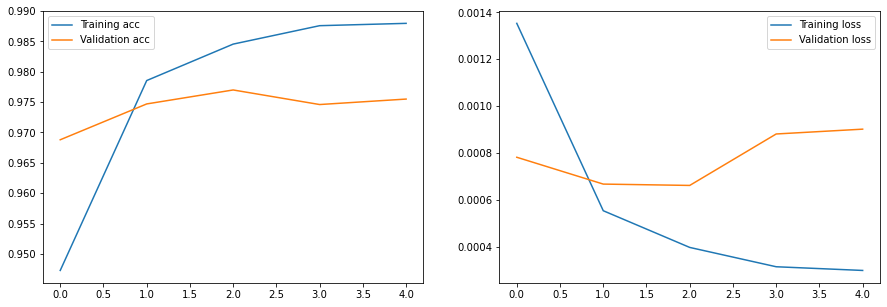
\includegraphics[width=0.9\linewidth,keepaspectratio]{pyt52}
\end{center}


As you can see, we are able to achieve higher accuracy, and much faster, compared to the fully-connected networks from previous unit.

\tiny{(Ref: Microsoft - Intro to Machine Learning using Pytorch)}

\begin{lstlisting}
hist = train(net,train_loader,test_loader,epochs=5)
plot_results(hist)
\end{lstlisting}

\end{frame}

%%%%%%%%%%%%%%%%%%%%%%%%%%%%%%%%%%%%%%%%%%%%%%%%%%%
\begin{frame}[fragile] \frametitle{Visualize Convolutional Layers}

We can also visualize the weights of our trained convolutional layers, to try and make some more sense of what is going on:



\begin{center}

\includegraphics[width=0.9\linewidth,keepaspectratio]{pyt53}
\end{center}


You can see that some of those filters look like they can recognize some oblique strokes, while others look pretty random.

\tiny{(Ref: Microsoft - Intro to Machine Learning using Pytorch)}


\begin{lstlisting}
fig,ax = plt.subplots(1,9)
with torch.no_grad():
    p = next(net.conv.parameters())
    for i,x in enumerate(p):
        ax[i].imshow(x.detach().cpu()[0,...])
        ax[i].axis('off')
\end{lstlisting}
\end{frame}


%%%%%%%%%%%%%%%%%%%%%%%%%%%%%%%%%%%%%%%%%%%%%%%%%%%
\begin{frame}[fragile] \frametitle{Multi-layered CNNs and pooling layers}

\begin{itemize}

\item First convolutional layers looks for primitive patterns, such as horizontal or vertical lines, but we can apply further convolutional layers on top of them to look for higher-level patterns, such as primitive shapes. 
\item Then more convolutional layers can combine those shapes into some parts of the picture, up to the final object that we are trying to classify.
\item We may also apply one trick: reducing the spatial size of the image. Once we have detected there is a horizontal stoke within sliding $3x3$ window, it is not so important at which exact pixel it occurred. 
\item Thus we can ``scale down'' the size of the image, which is done using one of the pooling layers:
\begin{itemize}
\item Average Pooling takes a sliding window (for example, 2x2 pixels) and computes an average of values within the window
\item Max Pooling replaces the window with the maximum value. The idea behind max pooling is to detect a presence of a certain pattern within the sliding window.
\end{itemize}
\end{itemize}

\tiny{(Ref: Microsoft - Intro to Machine Learning using Pytorch)}
\end{frame}


%%%%%%%%%%%%%%%%%%%%%%%%%%%%%%%%%%%%%%%%%%%%%%%%%%%
\begin{frame}[fragile] \frametitle{Multi-layered CNNs and pooling layers}

\begin{itemize}

\item A typical CNN there would be several convolutional layers, with pooling layers in between them to decrease dimensions of the image. 
\item We would also increase the number of filters, because as patterns become more advanced - there are more possible interesting combinations that we need to be looking for.

\item Because of decreasing spatial dimensions and increasing feature/filters dimensions, this architecture is also called pyramid architecture.
\end{itemize}


\begin{center}
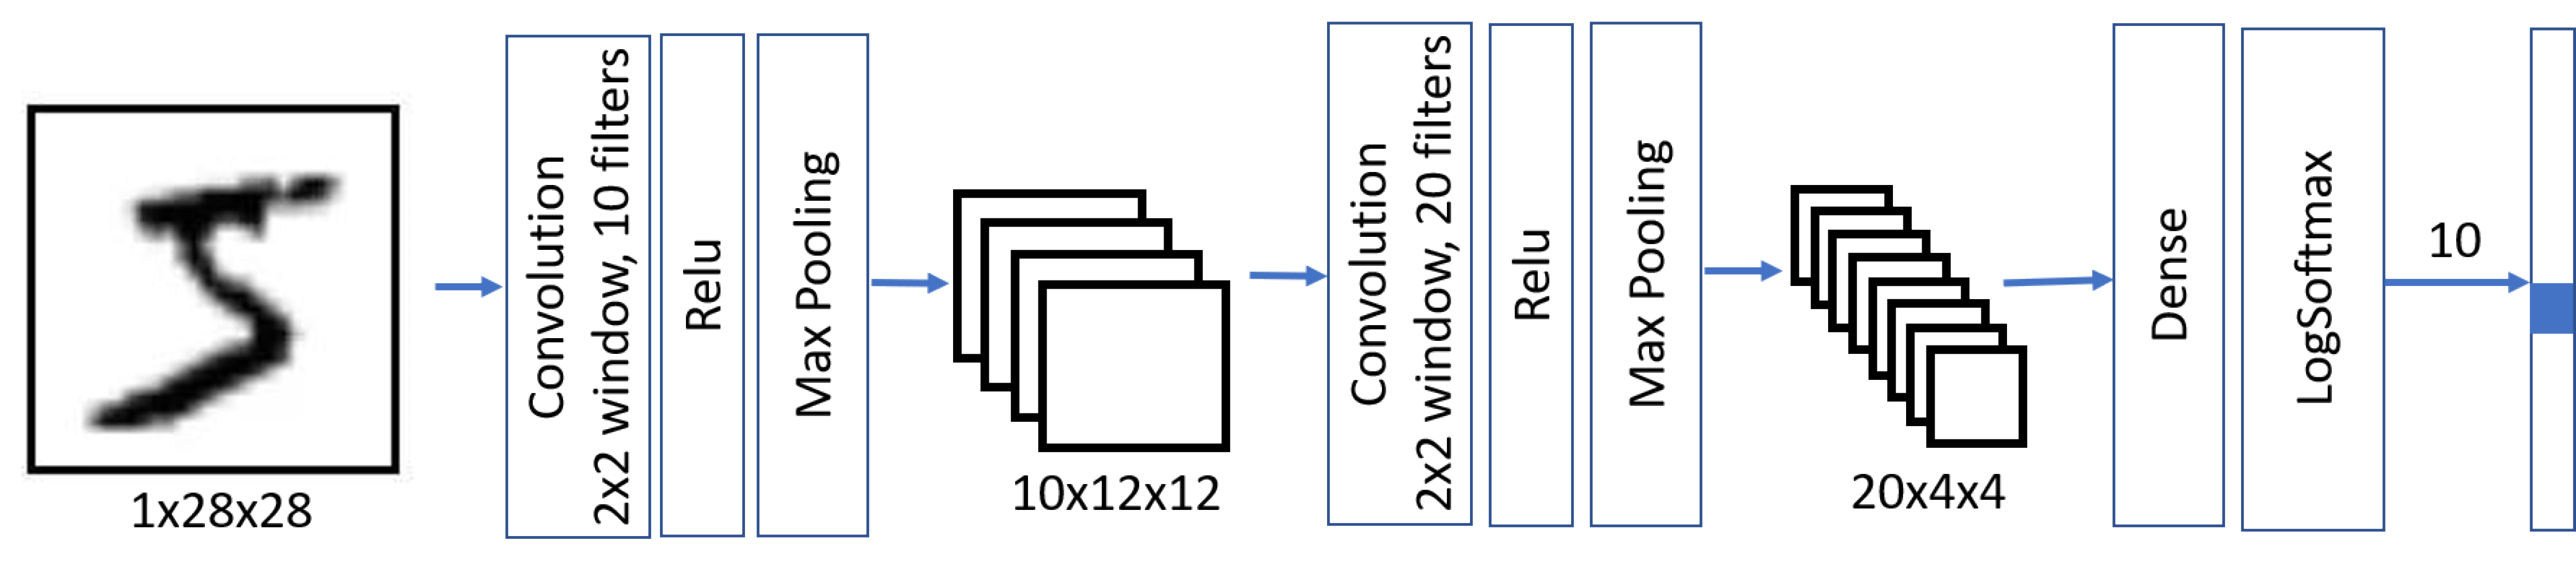
\includegraphics[width=0.9\linewidth,keepaspectratio]{pyt54}
\end{center}

\tiny{(Ref: Microsoft - Intro to Machine Learning using Pytorch)}
\end{frame}

%%%%%%%%%%%%%%%%%%%%%%%%%%%%%%%%%%%%%%%%%%%%%%%%%%%
\begin{frame}[fragile] \frametitle{Multi-layered CNNs and pooling layers}

\tiny{(Ref: Microsoft - Intro to Machine Learning using Pytorch)}

\begin{lstlisting}
class MultiLayerCNN(nn.Module):
    def __init__(self):
        super(MultiLayerCNN, self).__init__()
        self.conv1 = nn.Conv2d(1, 10, 5)
        self.pool = nn.MaxPool2d(2, 2)
        self.conv2 = nn.Conv2d(10, 20, 5)
        self.fc = nn.Linear(320,10)

    def forward(self, x):
        x = self.pool(nn.functional.relu(self.conv1(x)))
        x = self.pool(nn.functional.relu(self.conv2(x)))
        x = x.view(-1, 320)
        x = nn.functional.log_softmax(self.fc(x),dim=1)
        return x

net = MultiLayerCNN()
summary(net,input_size=(1,1,28,28))
\end{lstlisting}

\end{frame}

%%%%%%%%%%%%%%%%%%%%%%%%%%%%%%%%%%%%%%%%%%%%%%%%%%%
\begin{frame}[fragile] \frametitle{Multi-layered CNNs and pooling layers}

\begin{itemize}

\item Instead of using Flatten layer, we are flattening the tensor inside forward function using view function. Since flattening layer does not have trainable weights, no need to create a separate layer instance in constructor.
\item We use just one instance of pooling layer as it does not contain any trainable parameters, and this one can be reused
\item The number of trainable parameters (8.5K) is dramatically smaller than in previous cases. Small number of parameters have positive impact, because it helps to prevent overfitting even on smaller datasets.
\end{itemize}


\tiny{(Ref: Microsoft - Intro to Machine Learning using Pytorch)}

\begin{lstlisting}
==========================================================================
Layer (type:depth-idx)                   Output Shape              Param #
==========================================================================
|--Conv2d: 1-1                            [1, 10, 24, 24]           260
|--MaxPool2d: 1-2                         [1, 10, 12, 12]           -
|--Conv2d: 1-3                            [1, 20, 8, 8]             5,020
|--MaxPool2d: 1-4                         [1, 20, 4, 4]             -
|--Linear: 1-5                            [1, 10]                   3,210
==========================================================================
Total params: 8,490
Trainable params: 8,490
Non-trainable params: 0
Total mult-adds (M): 0.47
==========================================================================
\end{lstlisting}


\end{frame}

%%%%%%%%%%%%%%%%%%%%%%%%%%%%%%%%%%%%%%%%%%%%%%%%%%%
\begin{frame}[fragile] \frametitle{Multi-layered CNNs and pooling layers}

\begin{itemize}

\item We are able to achieve higher accuracy than with just one layer, and much faster - just with 1 or 2 epochs. 
\item It means that sophisticated network architecture needs much fewer data to figure out what is going on, and to extract generic patterns from our images.
\end{itemize}


\tiny{(Ref: Microsoft - Intro to Machine Learning using Pytorch)}

\begin{lstlisting}
hist = train(net,train_loader,test_loader,epochs=5)

>>>
Epoch  0, Train acc=0.952, Val acc=0.977, Train loss=0.001, Val loss=0.001
Epoch  1, Train acc=0.982, Val acc=0.983, Train loss=0.000, Val loss=0.000
Epoch  2, Train acc=0.986, Val acc=0.983, Train loss=0.000, Val loss=0.000
Epoch  3, Train acc=0.986, Val acc=0.978, Train loss=0.000, Val loss=0.001
Epoch  4, Train acc=0.987, Val acc=0.981, Train loss=0.000, Val loss=0.000
\end{lstlisting}


\end{frame}


% %%%%%%%%%%%%%%%%%%%%%%%%%%%%%%%%%%%%%%%%%%%%%%%%%%%
% \begin{frame}[fragile] \frametitle{CNN}
% \begin{center}
% \includegraphics[width=0.8\linewidth,keepaspectratio]{pyhun42}
% \end{center}
% First few layers are convoution+subsampling and at the end dense
% \end{frame}


% %%%%%%%%%%%%%%%%%%%%%%%%%%%%%%%%%%%%%%%%%%%%%%%%%%%
% \begin{frame}[fragile] \frametitle{Convolution}
% \begin{center}
% \includegraphics[width=0.8\linewidth,keepaspectratio]{pyhun43}
% \end{center}
% Looking at small portion of image, generating feature maps, one for each filter.
% \end{frame}

% %%%%%%%%%%%%%%%%%%%%%%%%%%%%%%%%%%%%%%%%%%%%%%%%%%%
% \begin{frame}[fragile] \frametitle{Convolution}
% \begin{center}
% \includegraphics[width=0.8\linewidth,keepaspectratio]{pyhun44}
% \end{center}
% First layer had 6 filters and the second has 10.
% \end{frame}


% %%%%%%%%%%%%%%%%%%%%%%%%%%%%%%%%%%%%%%%%%%%%%%%%%%%
% \begin{frame}[fragile] \frametitle{Pooling/Sub-sampling}
% \begin{center}
% \includegraphics[width=0.8\linewidth,keepaspectratio]{pyhun45}
% \end{center}

% \end{frame}


% %%%%%%%%%%%%%%%%%%%%%%%%%%%%%%%%%%%%%%%%%%%%%%%%%%%
% \begin{frame}[fragile] \frametitle{Difference}
% \begin{center}
% \includegraphics[width=0.8\linewidth,keepaspectratio]{pyhun46}
% \end{center}
% CNN is more flexible as it looks are smaller data, so smaller weights.
% \end{frame}


% %%%%%%%%%%%%%%%%%%%%%%%%%%%%%%%%%%%%%%%%%%%%%%%%%%%
% \begin{frame}[fragile] \frametitle{Simple CNN for MNIST}
% \begin{center}
% \includegraphics[width=0.8\linewidth,keepaspectratio]{pyhun47}
% \end{center}
% Using ready Conv2d layer with 1 input channel (greyscale), output channel = 10 (labels).
% \end{frame}


% %%%%%%%%%%%%%%%%%%%%%%%%%%%%%%%%%%%%%%%%%%%%%%%%%%%
% \begin{frame}[fragile] \frametitle{Simple CNN for MNIST}
% \begin{center}
% \includegraphics[width=0.8\linewidth,keepaspectratio]{pyhun48}
% \end{center}

% Outputs and Inputs need to be adjusted properly.  Calculating size after second pooling is not trivial, so just put some value and run. You will get error, suggesting a correct value. 64 is batch size, 320 is the flattened vector. Put 320 there.
% \end{frame}

% %%%%%%%%%%%%%%%%%%%%%%%%%%%%%%%%%%%%%%%%%%%%%%%%%%%
% \begin{frame}[fragile] \frametitle{Simple CNN for MNIST}
% \begin{center}
% \includegraphics[width=\linewidth,keepaspectratio]{pyhun49}
% \end{center}


% \end{frame}






%%%%%%%%%%%%%%%%%%%%%%%%%%%%%%%%%%%%%%%%%%%%%%%%%%%
\begin{frame}
  \begin{center}
    {\Large CNN using PyTorch: Comprehensive}
    
\tiny{(Ref: Pytorch Official documentation + few other sources, like Lyman Lin (NTU)))}
  \end{center}
\end{frame}



%%%%%%%%%%%%%%%%%%%%%%%%%%%%%%%%%%%%%%%%%%%%%%%%%%%
\begin{frame}[fragile] \frametitle{How CNN Works}
\begin{center}
\includegraphics[width=0.8\linewidth,keepaspectratio]{pyt20}
\end{center}

\end{frame}

%%%%%%%%%%%%%%%%%%%%%%%%%%%%%%%%%%%%%%%%%%%%%%%%%%%
\begin{frame}[fragile] \frametitle{How CNN Works}
\begin{center}
\includegraphics[width=0.8\linewidth,keepaspectratio]{pyt21}
\end{center}

\end{frame}

%%%%%%%%%%%%%%%%%%%%%%%%%%%%%%%%%%%%%%%%%%%%%%%%%%%
\begin{frame}[fragile] \frametitle{How CNN Works}
\begin{center}
\includegraphics[width=0.8\linewidth,keepaspectratio]{pyt22}
\end{center}

\end{frame}

%%%%%%%%%%%%%%%%%%%%%%%%%%%%%%%%%%%%%%%%%%%%%%%%%%%
\begin{frame}[fragile] \frametitle{How CNN Works}
\begin{center}
\includegraphics[width=0.8\linewidth,keepaspectratio]{pyt23}
\end{center}

\end{frame}

%%%%%%%%%%%%%%%%%%%%%%%%%%%%%%%%%%%%%%%%%%%%%%%%%%%
\begin{frame}[fragile] \frametitle{How CNN Works}
\begin{center}
\includegraphics[width=0.8\linewidth,keepaspectratio]{pyt24}
\end{center}

\end{frame}

%%%%%%%%%%%%%%%%%%%%%%%%%%%%%%%%%%%%%%%%%%%%%%%%%%%
\begin{frame}[fragile] \frametitle{How CNN Works}
\begin{center}
\includegraphics[width=0.8\linewidth,keepaspectratio]{pyt25}
\end{center}

\end{frame}

%%%%%%%%%%%%%%%%%%%%%%%%%%%%%%%%%%%%%%%%%%%%%%%%%%%
\begin{frame}[fragile] \frametitle{How CNN Works}
\begin{center}
\includegraphics[width=0.8\linewidth,keepaspectratio]{pyt26}
\end{center}

\end{frame}

%%%%%%%%%%%%%%%%%%%%%%%%%%%%%%%%%%%%%%%%%%%%%%%%%%%
\begin{frame}[fragile] \frametitle{How CNN Works}
\begin{center}
\includegraphics[width=0.8\linewidth,keepaspectratio]{pyt27}
\end{center}

\end{frame}


%%%%%%%%%%%%%%%%%%%%%%%%%%%%%%%%%%%%%%%%%%%%%%%%%%%
\begin{frame}[fragile] \frametitle{How CNN Works}
\begin{center}
\includegraphics[width=0.8\linewidth,keepaspectratio]{pyt28}
\end{center}

\end{frame}
%%%%%%%%%%%%%%%%%%%%%%%%%%%%%%%%%%%%%%%%%%%%%%%%%%%
\begin{frame}[fragile] \frametitle{How CNN Works}
\begin{center}
\includegraphics[width=0.8\linewidth,keepaspectratio]{pyt29}
\end{center}

\end{frame}


%%%%%%%%%%%%%%%%%%%%%%%%%%%%%%%%%%%%%%%%%%%%%%%%%%%
\begin{frame}[fragile] \frametitle{How CNN Works}
\begin{center}
\includegraphics[width=0.8\linewidth,keepaspectratio]{pyt6}
\end{center}

\end{frame}

%%%%%%%%%%%%%%%%%%%%%%%%%%%%%%%%%%%%%%%%%%%%%%%%%%%
\begin{frame}[fragile] \frametitle{How CNN Works}
\begin{center}
\includegraphics[width=0.8\linewidth,keepaspectratio]{pyt7}
\end{center}

\end{frame}


%%%%%%%%%%%%%%%%%%%%%%%%%%%%%%%%%%%%%%%%%%%%%%%%%%%
\begin{frame}[fragile] \frametitle{Define the network}
\begin{lstlisting}
import torch
from torch.autograd import Variable
import torch.nn as nn
import torch.nn.functional as F

class Net(nn.Module):
	pass
	
net = Net()
print(net)
\end{lstlisting}
\end{frame}

%%%%%%%%%%%%%%%%%%%%%%%%%%%%%%%%%%%%%%%%%%%%%%%%%%%
\begin{frame}[fragile] \frametitle{Define the network}
\begin{lstlisting}
class Net(nn.Module):

    def __init__(self):
        super(Net, self).__init__()
        # 1 input image channel, 6 output channels, 5x5 square convolution
        # kernel
        self.conv1 = nn.Conv2d(1, 6, 5)
        self.conv2 = nn.Conv2d(6, 16, 5)
        # an affine operation: y = Wx + b
        self.fc1 = nn.Linear(16 * 5 * 5, 120)
        self.fc2 = nn.Linear(120, 84)
        self.fc3 = nn.Linear(84, 10)
\end{lstlisting}
\end{frame}



%%%%%%%%%%%%%%%%%%%%%%%%%%%%%%%%%%%%%%%%%%%%%%%%%%%
\begin{frame}[fragile] \frametitle{Define the network}
\begin{lstlisting}
class Net(nn.Module):

    def forward(self, x):
        # Max pooling over a (2, 2) window
        x = F.max_pool2d(F.relu(self.conv1(x)), (2, 2))
        # If the size is a square you can only specify a single number
        x = F.max_pool2d(F.relu(self.conv2(x)), 2)
        x = x.view(-1, self.num_flat_features(x))
        x = F.relu(self.fc1(x))
        x = F.relu(self.fc2(x))
        x = self.fc3(x)
        return x
\end{lstlisting}
\end{frame}

%%%%%%%%%%%%%%%%%%%%%%%%%%%%%%%%%%%%%%%%%%%%%%%%%%%
\begin{frame}[fragile] \frametitle{How CNN Works}
\begin{center}
\includegraphics[width=0.8\linewidth,keepaspectratio]{pyt8}
\end{center}

\end{frame}

%%%%%%%%%%%%%%%%%%%%%%%%%%%%%%%%%%%%%%%%%%%%%%%%%%%
\begin{frame}[fragile] \frametitle{How CNN Works}
\begin{center}
\includegraphics[width=0.8\linewidth,keepaspectratio]{pyt9}
\end{center}

\end{frame}

%%%%%%%%%%%%%%%%%%%%%%%%%%%%%%%%%%%%%%%%%%%%%%%%%%%
\begin{frame}[fragile] \frametitle{How CNN Works}
\begin{center}
\includegraphics[width=0.8\linewidth,keepaspectratio]{pyt10}
\end{center}

\end{frame}

%%%%%%%%%%%%%%%%%%%%%%%%%%%%%%%%%%%%%%%%%%%%%%%%%%%
\begin{frame}[fragile] \frametitle{How CNN Works}
\begin{center}
\includegraphics[width=0.8\linewidth,keepaspectratio]{pyt11}
\end{center}

\end{frame}

%%%%%%%%%%%%%%%%%%%%%%%%%%%%%%%%%%%%%%%%%%%%%%%%%%%
\begin{frame}[fragile] \frametitle{How CNN Works}
\begin{center}
\includegraphics[width=0.8\linewidth,keepaspectratio]{pyt12}
\end{center}

\end{frame}

%%%%%%%%%%%%%%%%%%%%%%%%%%%%%%%%%%%%%%%%%%%%%%%%%%%
\begin{frame}[fragile] \frametitle{How CNN Works}
\begin{center}
\includegraphics[width=0.8\linewidth,keepaspectratio]{pyt13}
\end{center}

\end{frame}

%%%%%%%%%%%%%%%%%%%%%%%%%%%%%%%%%%%%%%%%%%%%%%%%%%%
\begin{frame}[fragile] \frametitle{How CNN Works}
\begin{center}
\includegraphics[width=0.8\linewidth,keepaspectratio]{pyt14}
\end{center}

\end{frame}

%%%%%%%%%%%%%%%%%%%%%%%%%%%%%%%%%%%%%%%%%%%%%%%%%%%
\begin{frame}[fragile] \frametitle{How CNN Works}
\begin{center}
\includegraphics[width=0.8\linewidth,keepaspectratio]{pyt15}
\end{center}

\end{frame}

%%%%%%%%%%%%%%%%%%%%%%%%%%%%%%%%%%%%%%%%%%%%%%%%%%%
\begin{frame}[fragile] \frametitle{How CNN Works}
\begin{center}
\includegraphics[width=0.8\linewidth,keepaspectratio]{pyt16}
\end{center}

\end{frame}

%%%%%%%%%%%%%%%%%%%%%%%%%%%%%%%%%%%%%%%%%%%%%%%%%%%
\begin{frame}[fragile] \frametitle{How CNN Works}
\begin{center}
\includegraphics[width=0.8\linewidth,keepaspectratio]{pyt17}
\end{center}

\end{frame}

%%%%%%%%%%%%%%%%%%%%%%%%%%%%%%%%%%%%%%%%%%%%%%%%%%%
\begin{frame}[fragile] \frametitle{How CNN Works}
\begin{center}
\includegraphics[width=0.8\linewidth,keepaspectratio]{pyt18}
\end{center}

\end{frame}

%%%%%%%%%%%%%%%%%%%%%%%%%%%%%%%%%%%%%%%%%%%%%%%%%%%
\begin{frame}[fragile] \frametitle{How CNN Works}
\begin{center}
\includegraphics[width=0.8\linewidth,keepaspectratio]{pyt19}
\end{center}
\tiny{(Reference:PyTorch Tutorial-NTU Machine Learning Course-Lyman Lin )}
\end{frame}
